\documentclass[12pt,a4paper]{article}
\usepackage[utf8]{inputenc}
\usepackage{graphicx}
\graphicspath{{../Images/}}
\usepackage{amsmath}
\usepackage{amsfonts}
\usepackage{amssymb}
\usepackage{hyperref}
\usepackage[margin=1in]{geometry}
\usepackage{subfig}
\usepackage{float}
\usepackage{xcolor}
\usepackage{listings}
\definecolor{dkgreen}{rgb}{0,0.6,0}
\definecolor{gray}{rgb}{0.5,0.5,0.5}
\definecolor{mauve}{rgb}{0.58,0,0.82}

\lstset{frame=tb,
  language=Python,
  aboveskip=3mm,
  belowskip=3mm,
  showstringspaces=false,
  columns=flexible,
  basicstyle={\small\ttfamily},
  numbers=none,
  numberstyle=\tiny\color{gray},
  keywordstyle=\color{blue},
  commentstyle=\color{dkgreen},
  stringstyle=\color{mauve},
  breaklines=true,
  breakatwhitespace=true,
  tabsize=3
}

\author{Thibaut Marmey}

\title{Notes de cours CADL - session-1\\
\normalsize \href{https://www.kadenze.com/courses/creative-applications-of-deep-learning-with-tensorflow-iv/sessions/introduction-to-tensorflow}{cours Kadenze - session-1}}

\begin{document}
	\maketitle

\begin{scriptsize} \begin{itemize}
\item Learn the basic idea behind machine learning: learning from data and discovering representations
\item Learn how to preprocess a dataset using its mean and standard deviation
\item Learn the basic components of a Tensorflow Graph
\end{itemize}\end{scriptsize}

\begin{normalsize}
\tableofcontents
\end{normalsize}

\section{Introduction}
\subsection{Généralités}
\begin{itemize}
\item Deep-learning in a type of Machine Learning
\item \textit{Deep} because it is composed of many layers of \textit{Neural Networks}
\item Other valuable branches of Machine Learning :
\begin{itemize}
\item Rinforcement Learning
\item Dictionary Learning
\item Probabilistic Graphical Models and Bayesian Methods (Bishop)
\item Genetic and Evolutionary Algorithms
\end{itemize}
\item The differents ways an object can appear in an image is called \textit{invariance}
\item The dataset teaches the algorithm how to see the world, but only the world of this dataset
\item Existing data :
\begin{itemize}
\item MNIST
\item CalTech
\item CelebNet
\item \href{http://www.image-net.org/}{ImageNet}
\item LFW
\item CIFAR10, CIFRA100, \href{http://mscoco.org/home/}{MS Coco}...
\end{itemize}
\end{itemize}


\subsection{Preprocessing Data}
\begin{itemize}
\item Collect the images into a batch configuration. With this configuration, it's easier to make some computation over all the data.\\
This means, the data is in a single \textit{numpy} variable : \textit{data = np.array(imgs)}
\item Compute the Mean and Deviation of Images (of the batch channel)
\begin{itemize}
\item \begin{lstlisting}
mean_img = np.mean(data, axis=0) #mean of each col
plt.imshow(mean_img.astype(np.uint8))
\end{lstlisting}
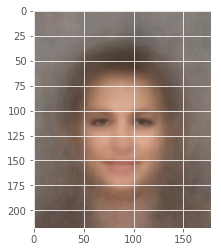
\includegraphics[scale=0.5]{dataMean}\\
This describes what most the dataset looks like.
\item \begin{lstlisting}
std_img = np.std(data, axis=0)
plt.imshow(std_img.astype(np.uint8))
\end{lstlisting}
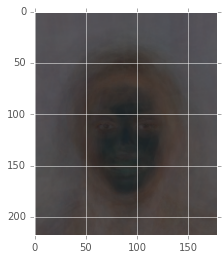
\includegraphics[scale=0.5]{dataStd}\\
This describes where the changes are the most likely to appear in the dataset of images.
\item \begin{lstlisting}
plt.imshow(np.mean(std_img, axis=2).astype(np.uint8))
\end{lstlisting}
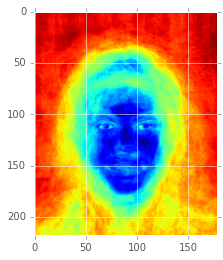
\includegraphics[scale=0.5]{dataStdMean}\\
This describes how every color channel will vary as a heatmap.
\begin{itemize}
\item Red part : not the best representation of the image
\item Blue part : the less likely that our mean image is far off from any other possible image
\end{itemize}
\end{itemize}
\end{itemize}

\subsection{Dataset preprocessing}
\begin{itemize}
\item We are trying to build a model that understands invariances (different of vision of an object, localization in the image, etc...)
\item If we use DL to learn something complex in the data, it starts by modeling both the mean and standard deviation or our dataset.
\item Speed up by "preprocessing" the dataset by removing the mean and standard deviation : it's called \textit{normalization}.\\
Subsctracting the mean and dividing by the standard deviation.
\item Look at the dataset with another way : array into a 1 dimensional array.
\begin{lstlisting}
flattened = data.ravel()
\end{lstlisting}
\item Visualize the \textbf{"distribution"}, or range and frequence of possible values. This tell us if \textbf{the data is predictable or not}.\\
\textit{plt.hist(data.ravel(), n} takes the min and max values of the \textit{data} array, and divide this interval in \textit{n} subintervals.
\begin{lstlisting}
plt.hist(flattened.ravel(), 255) #values are grouping in 255 bins
\end{lstlisting}
It tells us if something seems to happen more than anything else. If it does, the neural network will take advantage of that.
\item Normalization :
\begin{lstlisting}
plt.hist(((data[0] - mean_img) / std_img).ravel(), bins)
\end{lstlisting}
The data has been squished into a peak. Change the scale of the hist.\\
The data is concentrated between two values. The effect of normalizing : most of the data will be around 0, where some deviations of it will follow between the two values.\\
\begin{minipage}{\linewidth}
  \begin{figure}[H]
  \centering
    \subfloat[]{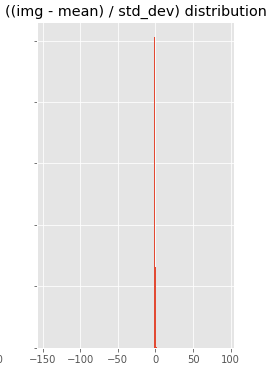
\includegraphics[scale=0.4]{normalizationPeak}}\hspace{1cm}
    \subfloat[]{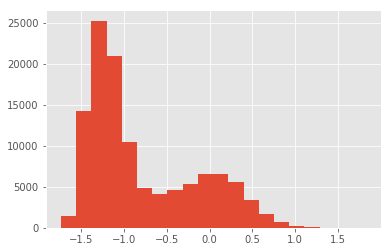
\includegraphics[scale=0.4]{normalizationPeakScaled}}
  \end{figure}
\end{minipage}
\item If the normalization doesn't look like this :
\begin{itemize}
\item get more data to calculate our mean/std deviation
\item try another method of normalization
\item not bother with normalization at all
\end{itemize}
\item Other options of normalization :
\begin{itemize}
\item local contrast normalization for images
\item PCA based normalization
\end{itemize}
\end{itemize}


\end{document}